\documentclass[10pt,aspectratio=169]{beamer}

% Inspired by the practical Beamer setup in Joonas Laukka's
% Helsinki Haskell Meetup presentation-without-notes.tex.
\usetheme{Copenhagen}
\beamertemplatenavigationsymbolsempty
\setbeamertemplate{caption}[numbered]

\usepackage[T1]{fontenc}
\usepackage[utf8]{inputenc}
\usepackage{lmodern}
\usepackage{graphicx}
\usepackage{listings}
\usepackage{xcolor}
\usepackage{microtype}
\usepackage{ragged2e}

\renewcommand{\familydefault}{\sfdefault}

\definecolor{DeckBackground}{HTML}{EAF5FF}
\definecolor{DeckText}{HTML}{102A43}
\definecolor{DeckMuted}{HTML}{486581}
\definecolor{DeckAccent}{HTML}{006D9C}
\definecolor{DeckRed}{HTML}{B42318}
\definecolor{DeckBlue}{HTML}{0077B6}
\definecolor{CodeBackground}{HTML}{D8ECFA}

\setbeamercolor{normal text}{fg=DeckText,bg=DeckBackground}
\setbeamercolor{structure}{fg=DeckAccent}
\setbeamercolor{frametitle}{fg=DeckText,bg=DeckBackground}
\setbeamercolor{title}{fg=DeckText}
\setbeamercolor{subtitle}{fg=DeckMuted}
\setbeamercolor{author}{fg=DeckText}
\setbeamercolor{institute}{fg=DeckMuted}
\setbeamercolor{date}{fg=DeckMuted}
\setbeamercolor{itemize item}{fg=DeckAccent}
\setbeamercolor{itemize subitem}{fg=DeckBlue}

\setbeamerfont{title}{size=\fontsize{28}{31}\selectfont,series=\bfseries}
\setbeamerfont{subtitle}{size=\large}
\setbeamerfont{frametitle}{size=\fontsize{22}{25}\selectfont,series=\bfseries}
\setbeamerfont{normal text}{size=\large}
\setbeamersize{text margin left=8mm,text margin right=8mm}
\setbeamertemplate{headline}{}
\setbeamertemplate{frametitle}{%
  \vspace{4mm}\hspace{1mm}\insertframetitle\par\vspace{2mm}
}
\setbeamertemplate{footline}{%
  \hfill{\color{DeckMuted}\scriptsize\insertframenumber}\hspace{6mm}\vspace{3mm}
}

\lstdefinestyle{deckcode}{
  basicstyle=\ttfamily\small\color{DeckText},
  backgroundcolor=\color{CodeBackground},
  frame=single,
  rulecolor=\color{CodeBackground},
  framesep=5pt,
  xleftmargin=3pt,
  xrightmargin=3pt,
  columns=fullflexible,
  keepspaces=true,
  showstringspaces=false,
  breaklines=true,
  tabsize=2,
  keywordstyle=\color{DeckAccent}\bfseries,
  commentstyle=\color{DeckMuted},
  stringstyle=\color{DeckBlue}
}

\newcommand{\accentline}[1]{{\color{DeckAccent}\bfseries #1}}
\newcommand{\muted}[1]{{\color{DeckMuted}#1}}
\newcommand{\danger}[1]{{\color{DeckRed}\bfseries #1}}
\newcommand{\blueline}[1]{{\color{DeckBlue}\bfseries #1}}
\newcommand{\bottomline}[2][DeckAccent]{%
  \vfill{\color{#1}\large\bfseries #2}\par
}

\title{Encoding Intent:\\Type-Driven Development in the Age of AI}
\subtitle{Types and evidence across trust boundaries}
\author{Joonas Laukka}
\institute{Senior Consultant at Loihde}
\date{}

\begin{document}

{\setbeamertemplate{footline}{}
\begin{frame}[plain]
  \begin{columns}[T,onlytextwidth]
    \begin{column}{0.58\textwidth}
      \vspace{10mm}
      {\color{DeckAccent}\fontsize{25}{28}\selectfont\bfseries Encoding Intent:}\par
      \vspace{2mm}
      {\color{DeckText}\fontsize{29}{32}\selectfont\bfseries
        Type-Driven\\Development\\in the Age of AI}\par
      \vspace{7mm}
      {\color{DeckMuted}\large Types and evidence across trust boundaries}\par
      \vfill
      {\large\bfseries Joonas Laukka}\par
      {\color{DeckMuted}Senior Consultant at Loihde}
    \end{column}
    \begin{column}{0.38\textwidth}
      \centering
      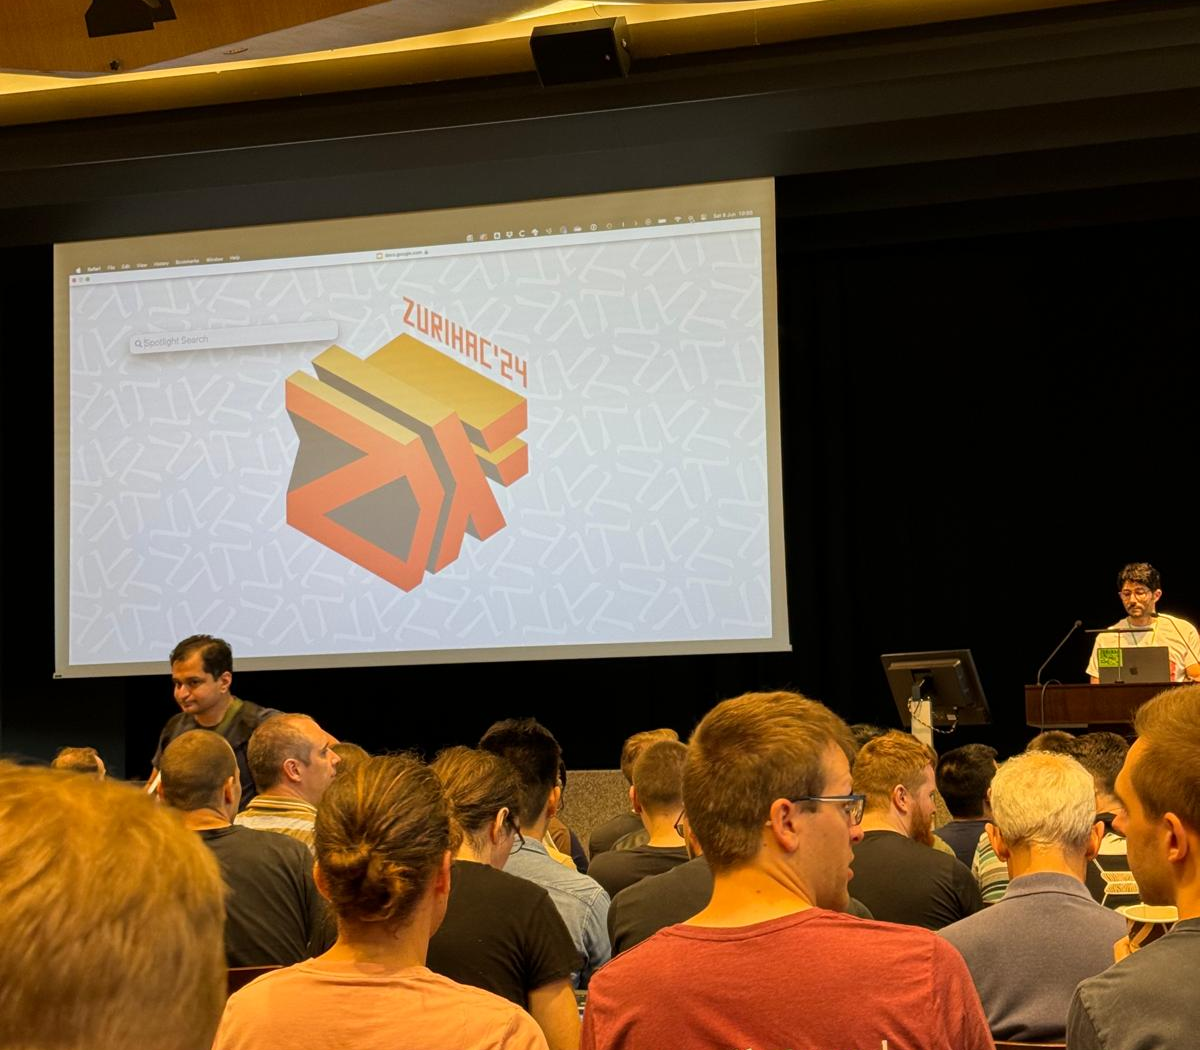
\includegraphics[width=\linewidth,height=.52\paperheight,keepaspectratio]{assets/zurihac-stage.png}\par
      \vspace{3mm}
      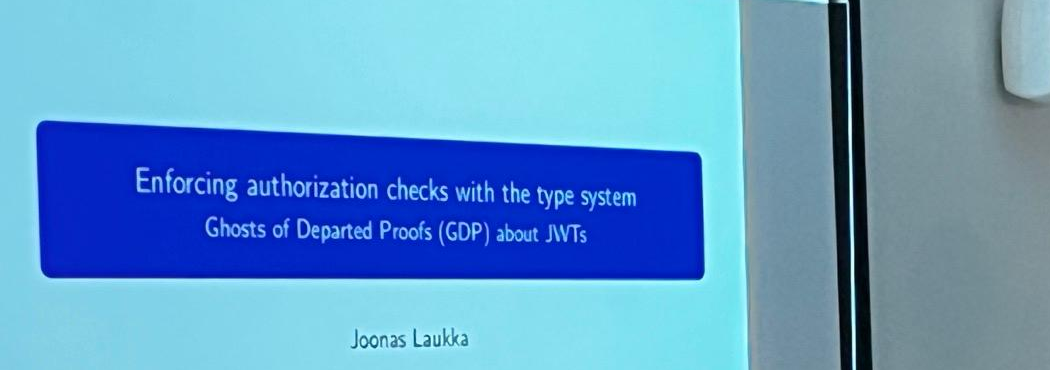
\includegraphics[width=\linewidth,height=.17\paperheight,keepaspectratio]{assets/talk-title.png}
    \end{column}
  \end{columns}
\end{frame}}

\begin{frame}[t]{Types narrow the space of possible programs}
  \mbox{}\par
  {\bfseries A signature documents what a function accepts and promises to return.}\par
  \vspace{3mm}
  {\color{DeckMuted}\large All syntactically valid programs}\par
  \vspace{3mm}\hspace{10mm}{\color{DeckBlue}\large\bfseries Well-typed programs}\par
  \vspace{3mm}\hspace{22mm}{\color{DeckAccent}\large\bfseries Programs satisfying domain-specific types}\par
  \vspace{5mm}
  {\small\muted{A type system can reject only the violations its types express.}}
\end{frame}

\begin{frame}[fragile]{Typed holes expose the remaining problem}
  \begin{columns}[T,onlytextwidth]
    \begin{column}{0.53\textwidth}
      \accentline{Incomplete program}
\begin{lstlisting}[style=deckcode,language=Haskell]
transform :: (a -> b) -> Maybe a -> Maybe b

transform _ Nothing  = Nothing
transform f (Just x) = Just _
\end{lstlisting}
    \end{column}
    \begin{column}{0.42\textwidth}
      \blueline{Compiler response}
\begin{lstlisting}[style=deckcode]
Found hole: _ :: b

Relevant bindings:
  f :: a -> b
  x :: a
\end{lstlisting}
    \end{column}
  \end{columns}
  \vfill
  {\color{DeckAccent}\Large\bfseries The hole asks: what value of type \texttt{b} can be built here?}\par
  \muted{The available function and value make \texttt{f x} the obvious candidate.}
\end{frame}

\begin{frame}[fragile]{Types turn implementation into constrained search}
\begin{lstlisting}[style=deckcode,language=Haskell]
transform f (Just x) = Just (f x)
\end{lstlisting}
  \vspace{5mm}
  {\color{DeckAccent}\fontsize{23}{27}\selectfont\bfseries
  Could a human-written type signature\\guide an AI agent in the same way?}\par
  \vfill
  \danger{An agent can also modify the types.}\par
  \vspace{2mm}
  \muted{The signature creates guidance and review pressure.\\
  The surrounding workflow must protect the contract.}
\end{frame}

\begin{frame}{An LLM-bound field can grow without a limit}
  \vspace{8mm}
  {\Large\bfseries An agent adds \texttt{streetAddress?: string | null}}\par
  \vspace{12mm}
  {\color{DeckMuted}\Large The request still looks valid to TypeScript.}\par
  \vspace{13mm}
  {\color{DeckAccent}\fontsize{24}{28}\selectfont\bfseries Which test now has to change?}
\end{frame}

\begin{frame}[fragile]{Derive the fields requiring an abuse test}
\begin{lstlisting}[style=deckcode,language=Java]
type StringLikeKey = {
  [K in keyof AiSearchFilters]-?:
    NonNullable<AiSearchFilters[K]> extends string | string[]
      ? K : never;
}[keyof AiSearchFilters];

// "query" | "city" | "postalCode"
\end{lstlisting}
  \bottomline{A new string field changes this union automatically.}
\end{frame}

\begin{frame}[fragile]{The type of an exhaustive test table}
\begin{lstlisting}[style=deckcode,language=Java]
type OverlongValue<K extends StringLikeKey> =
  NonNullable<AiSearchFilters[K]> extends string[]
    ? string[] : string;

type TestCases = {
  [K in StringLikeKey]: {
    maxLength: number;
    validValue: OverlongValue<K>;
    makeValue: (text: string) => OverlongValue<K>;
  };
};
\end{lstlisting}
  \bottomline{A new string field becomes a required test case.}
\end{frame}

\begin{frame}[fragile]{The complete test-case table}
\begin{lstlisting}[style=deckcode,language=Java,basicstyle=\ttfamily\footnotesize\color{DeckText}]
const cases = {
  query: {
    maxLength: 120, validValue: ["ok"],
    makeValue: (s) => [s],
  },
  city: {
    maxLength: 120, validValue: ["ok"],
    makeValue: (s) => [s],
  },
  postalCode: {
    maxLength: 10, validValue: "00100",
    makeValue: (s) => s,
  },
} satisfies TestCases;
\end{lstlisting}
  \bottomline{Omit \texttt{postalCode} and TypeScript points at the gap.}
\end{frame}

\begin{frame}[fragile]{Then test the runtime boundary}
\begin{lstlisting}[style=deckcode,language=Java]
for (const [key, c] of Object.entries(cases)) {
  expect(parseRequest(
    withFilter(key, c.validValue)
  )).not.toBeNull();

  const tooLong = "a".repeat(c.maxLength + 1);
  expect(parseRequest(
    withFilter(key, c.makeValue(tooLong))
  )).toBeNull();
}
\end{lstlisting}
  \bottomline{Compiler: include a case. Test: the parser rejects it.}
\end{frame}

\begin{frame}{The boundary of that guarantee}
  \vspace{7mm}
  {\Large\bfseries New field}\par
  \vspace{7mm}
  {\color{DeckRed}\Large Missing test case: compile error}\par
  \vspace{7mm}
  {\color{DeckAccent}\Large Missing runtime limit: failing test}\par
  \vfill
  {\color{DeckMuted}\Large Other payload growth needs other limits.}
\end{frame}

\begin{frame}[fragile]{A value and its permit}
\begin{lstlisting}[style=deckcode,language=Java]
type DeletePermit = {
  readonly applicationId: ApplicationId;
  readonly [permitBrand]: true;
};

function deleteApplication(
  id: ApplicationId, permit: DeletePermit
): void;

deleteApplication(appB, permitForAppA); // type-checks
\end{lstlisting}
  \bottomline[DeckRed]{The permit has an ID. The signature cannot equate the two IDs.}
\end{frame}

\begin{frame}[fragile]{Give this value a fresh type-level name}
\begin{lstlisting}[style=deckcode,language=Haskell]
name :: a -> (forall name. a ~~ name -> t) -> t

name jwtA $ \namedA ->
  name jwtB $ \namedB ->
    -- namedA :: SignedJWT ~~ a
    -- namedB :: SignedJWT ~~ b
\end{lstlisting}
  \bottomline{The two names cannot be exchanged in well-typed code.}
\end{frame}

\begin{frame}[fragile]{A proof names the value it describes}
\begin{lstlisting}[style=deckcode,language=Haskell]
isPrime :: (Int ~~ n) -> Maybe (Proof (IsPrime n))

usePrime
  :: (Int ~~ n)
  -> Proof (IsPrime n)
  -> m ()

usePrime namedB proofForA  -- names do not unify
\end{lstlisting}
  \bottomline{“Prime” is a property of a particular named integer.}
\end{frame}

\begin{frame}[fragile]{Proofs cannot cross issuers}
\begin{lstlisting}[style=deckcode,language=Haskell]
getClaimsOf @"azure" namedJWT
  :: m (Maybe
       (ClaimsSet ~~ ClaimsOf token
         ::: (token `IssuedBy` "azure")))

hasAzureRole @"administrator" azureClaims
  :: Maybe
       (Proof (ClaimsOf token
         `HasAzureRole` "administrator"))
\end{lstlisting}
  \bottomline[DeckRed]{OKTA claims cannot satisfy the Azure role checker.}
\end{frame}

\begin{frame}[fragile]{Authorization becomes a proposition}
\begin{lstlisting}[style=deckcode,language=Haskell]
canDeleteApps :: Proof (
  (token `IssuedBy` "azure"
    && ClaimsOf token `HasAzureRole` "administrator")
  --> CanDeleteApps token
)

buildAuthorizationProof
  :: SignedJWT ~~ token
  -> m (Maybe (Proof (CanDeleteApps token)))
\end{lstlisting}
  \bottomline{The protected call requires \texttt{Proof (CanDeleteApps token)}.}
\end{frame}

\begin{frame}[fragile]{Carry an unknown name with its proof}
\begin{lstlisting}[style=deckcode,language=Haskell]
data AuthorizedJWT where
  AuthorizedJWT
    :: (SignedJWT ~~ token)
    -> Proof (CanDeleteApps token)
    -> AuthorizedJWT

useAuthorized (AuthorizedJWT jwt proof) =
  actAs jwt proof
  -- both arguments share hidden token
\end{lstlisting}
  \bottomline{Existential: the caller need not know the token name.}
\end{frame}

\begin{frame}[fragile]{Another route: typed logging}
\begin{lstlisting}[style=deckcode,language=Haskell]
logInfoF @"session %{SessionKey}" sessionKey

instance
  ( ToLog argument
  , LogTypeName argument ~ slotName
  , BuildLogFunction slotNames format m result
  ) => BuildLogFunction
         (slotName ': slotNames) format m
         (argument -> result)
\end{lstlisting}
  \bottomline{The format requires both a permitted value and the right slot.}
\end{frame}

\begin{frame}{Which guarantees are worth the machinery?}
  \vspace{5mm}
  {\Large Exhaustive tables require a maintenance decision.}\par
  \vspace{9mm}
  {\color{DeckAccent}\Large GDP relates evidence to a particular value.}\par
  \vspace{9mm}
  {\color{DeckBlue}\Large Runtime validation establishes the evidence.}\par
  \vfill
  {\color{DeckMuted}\Large Use the simplest contract that covers the risk.}
\end{frame}

\begin{frame}{A question for your next code change}
  \vspace{13mm}
  {\fontsize{29}{34}\selectfont\bfseries
  Which assumption should become\\a compiler error?}\par
  \vspace{16mm}
  {\color{DeckAccent}\Large\bfseries
  And what runtime check must make that error meaningful?}
\end{frame}

\end{document}
